\documentclass[russian,utf8,pointsection]{eskdtext}
\usepackage{eskdchngsheet}
\usepackage[T2A]{fontenc}
\usepackage{pscyr}
\usepackage{graphicx}
\usepackage{amstext}
\usepackage{amsmath}
\usepackage{listings}
\usepackage[unicode]{hyperref}
\usepackage{multirow}
\usepackage{listings}
\usepackage[utf8]{inputenc}
\usepackage[english,russian]{babel}

\graphicspath{{image/}}
\DeclareGraphicsExtensions{.pdf,.png,.jpg}


\ESKDdepartment{ГБОУ ВПО Нижегородский государственный технический университет им. Р. Е. Алексеева}
\ESKDcompany{Институт радиоэлектроники и информационных технологий, кафедра "Вычислительные системы и технологии"}
\ESKDtitle{Технологии распределённой обработки данных}
\ESKDdocName{Отчет к лабораторной работе №3}
\ESKDsignature{Распараллеливание алгоритма с помощью библиотеки CCR}
\ESKDauthor{Пономарёв~Е.~В.}
\ESKDtitleAgreedBy{Доцент каф. ВСТ}{Гай В. Е.}
\ESKDtitleDesignedBy{Студент гр. 13-В-1}{Пономарёв~Е.~В.}
\ESKDchecker{Гай В. Е.}
\ESKDdate{2015/12/16}

\begin{document}
	\maketitle
	\tableofcontents
	\newpage
	
	\section{Цель и порядок выполнения работы}
		  Цель работы: получить представления о возможностях используемой библиотеки Concurrent and Coordination Runtime для организации параллельных вычислений.
	
	Порядок выполнения работы:
	\begin{enumerate}
		\item Разработка последовательного алгоритма, решающего одну из приведённых задач в соответствии с выданным вариантом задания;
		\item Разработка параллельного алгоритма, соответствующий варианту последовательного алгоритма;
		\item Выполнение сравнения времени выполнения последовательного и параллельного алгоритмов обработки данных при различных размерностях исходных данных.
	\end{enumerate}
	\newpage 
	
	
	\lstset{
		breaklines=true, % Перенос длинных строк
		literate={а}{{\selectfont\char224}}1
		{б}{{\selectfont\char225}}1
		{в}{{\selectfont\char226}}1
		{г}{{\selectfont\char227}}1
		{д}{{\selectfont\char228}}1
		{е}{{\selectfont\char229}}1
		{ё}{{\"e}}1
		{ж}{{\selectfont\char230}}1
		{з}{{\selectfont\char231}}1
		{и}{{\selectfont\char232}}1
		{й}{{\selectfont\char233}}1
		{к}{{\selectfont\char234}}1
		{л}{{\selectfont\char235}}1
		{м}{{\selectfont\char236}}1
		{н}{{\selectfont\char237}}1
		{о}{{\selectfont\char238}}1
		{п}{{\selectfont\char239}}1
		{р}{{\selectfont\char240}}1
		{с}{{\selectfont\char241}}1
		{т}{{\selectfont\char242}}1
		{у}{{\selectfont\char243}}1
		{ф}{{\selectfont\char244}}1
		{х}{{\selectfont\char245}}1
		{ц}{{\selectfont\char246}}1
		{ч}{{\selectfont\char247}}1
		{ш}{{\selectfont\char248}}1
		{щ}{{\selectfont\char249}}1
		{ъ}{{\selectfont\char250}}1
		{ы}{{\selectfont\char251}}1
		{ь}{{\selectfont\char252}}1
		{э}{{\selectfont\char253}}1
		{ю}{{\selectfont\char254}}1
		{я}{{\selectfont\char255}}1
		{А}{{\selectfont\char192}}1
		{Б}{{\selectfont\char193}}1
		{В}{{\selectfont\char194}}1
		{Г}{{\selectfont\char195}}1
		{Д}{{\selectfont\char196}}1
		{Е}{{\selectfont\char197}}1
		{Ё}{{\"E}}1
		{Ж}{{\selectfont\char198}}1
		{З}{{\selectfont\char199}}1
		{И}{{\selectfont\char200}}1
		{Й}{{\selectfont\char201}}1
		{К}{{\selectfont\char202}}1
		{Л}{{\selectfont\char203}}1
		{М}{{\selectfont\char204}}1
		{Н}{{\selectfont\char205}}1
		{О}{{\selectfont\char206}}1
		{П}{{\selectfont\char207}}1
		{Р}{{\selectfont\char208}}1
		{С}{{\selectfont\char209}}1
		{Т}{{\selectfont\char210}}1
		{У}{{\selectfont\char211}}1
		{Ф}{{\selectfont\char212}}1
		{Х}{{\selectfont\char213}}1
		{Ц}{{\selectfont\char214}}1
		{Ч}{{\selectfont\char215}}1
		{Ш}{{\selectfont\char216}}1
		{Щ}{{\selectfont\char217}}1
		{Ъ}{{\selectfont\char218}}1
		{Ы}{{\selectfont\char219}}1
		{Ь}{{\selectfont\char220}}1
		{Э}{{\selectfont\char221}}1
		{Ю}{{\selectfont\char222}}1
		{Я}{{\selectfont\char223}}1
	}
	
	\lstset{
		language=Java,
		basicstyle=\footnotesize
	}
	
	
    \section{Теоретические сведения}
    \subsection{Библиотека Concurrent and Coordination Runtime}
    Библиотека Concurrent and Coordination Runtime (CCR) предназначена для организации обработки данных с помощью параллельно и асинхронно
    выполняющихся методов. Взаимодействие между такими методами организуется на основе сообщений. Рассылка сообщений основана на     использовании портов.
    Основные понятия CCR:
    \begin{enumerate}
    \item Сообщение – экземпляр любого типа данных;
    \item Порт – очередь сообщений типа FIFO (First-In-First-Out), сообщение остаётся в порте пока не будут извлечено из очереди порта     получателем.
    Определение порта:
    
    Port<int> p = new Port<int>();
    
    Отправка сообщения в порт:
    
    p.Post(1);
    
    \item получатель – структура, которая выполняет обработку сообщений.
    Данная структура объединяет:
    	\begin{itemize}
   \item один или несколько портов, в которые отправляются сообщения;
    \item метод (или методы), которые используются для обработки сообщений (такой метод называется задачей);
    \item логическое условие, определяющее ситуации, в которых активизируется тот или иной получатель.
    
    Делегат, входящий в получатель, выполнится, когда в порт intPort придёт сообщение.
    Получатели сообщений бывают двух типов: временные и постоянные (в примере получатель – временный). Временный получатель, обработав
    сообщение (или несколько сообщений), удаляется из списка получателей сообщений данного порта.
    \end{itemize}
        
    \item процессом запуска задач управляет диспетчер. После выполнения условий активации задачи (одним из условий активации может быть
    получение портом сообщения) диспетчер назначает задаче поток из пула потоков, в котором она будет выполняться.
    Описание диспетчера с двумя потоками в пуле:
    
    Dispatcher d = new Dispatcher(2, "MyPool");
    
    Описание очереди диспетчера, в которую задачи ставятся на выполнение:
    
    DispatcherQueue dq = new DispatcherQueue("MyQueue", d);
    
    \end{enumerate}
    
       \subsection{Создание проекта}
       Нужно выполнить следующие действия:
       \begin{enumerate}
       \item Установить библиотеку CCR (CCR входит в состав Microsoft Robotics Developer Studio);
       \item Создать проект консольного приложения и добавьте к проекту библиотеку Microsoft.Ccr.Core.dll.
       	\end{enumerate}
       	
       	\subsection{Оценка времени выполнения}
       	Время выполнения вычислений будем определять с помощью класса
       	\begin{lstlisting}
       	Stopwatch:       	
       	Stopwatch sWatch = new Stopwatch();       	
       	sWatch.Start();       	
       	<выполняемый код>       	
       	sWatch.Stop();       	
       	Console.WriteLine(sWatch.ElapsedMilliseconds.ToString());
       	      	\end{lstlisting}
       	
       	\section{Выполнение лабораторной работы}
       		\subsection{Вариант задания}
       		Вариант 18:
	       	Разработать алгоритм вычисления значения определённого интеграла с использованием метода Монте-Карло

       	\subsection{Особенности реализации}
       	В ходе выполнения лабораторной работы возникли некоторые сложности: получалось так, что подынтегральная функция задается в исходном коде программистом, а пользователь программы будет иметь возможность при каждом запуске программы считать лишь один и тот же интеграл. Мной было принято решение устранить эту проблему. Для этого я решил воспользоваться возможностями скриптового языка программирования Python, с помощью которого можно с легкостью реализовать ввод подынтегральной функции пользователем как строки, а затем преобразования введенной строки в исполняемый исходный код языка Python с помощью функции eval(). 
       	В разработанном модуле на языке Python содержатся две функции, реализующие ввод значений пользователем  param\_enter()  и само интегрирование методом Монте-Карло  monte\_carlo() , а так же код, тестирующий работу программы, но выполняющийся только когда модуль запущен как отдельный файл, а не вызван сторонним приложением.
       	После разработки и отладки модуля на Python, возник вопрос об осуществлении связи между модулем, написанным на C\#, и разработанным модулем на Python. Решением этого вопроса стала установка нескольких дополнительных пакетов с помощью менеджера NuGet, а именно:
       	
       	\begin{enumerate}
       		\item DynamicLanguageRuntime.1.1.0 - для создания и использования динамических объектов;
       		\item IronPython.2.7.5 - для взаимодействия со скриптами языка Python;
       		\item IronPython.StdLib.2.7.5 - для подключения стандартной библиотеки (нужна для использования random.py);
       	\end{enumerate} 
       	
       	Подробное описание механизма взаимодействия модулей C\# и Python дается в комментариях в соотвествующих местах листинга разработанных модулей.
       	       			
       	\subsection{Листинг программы}
       
  \subsubsection{Модуль C\#}   
  \lstinputlisting[language=Java]
   {Program.cs}
   
  \subsubsection{Модуль Python}
  \lstinputlisting[language=Python]
   {monte-carlo.py}
   .
       	
       	\subsection{Результат работы программы}
       	Скриншот работы программы представлен на Рис. \ref{ris:1_2}.
       	\begin{figure}[!h]
       		\centering{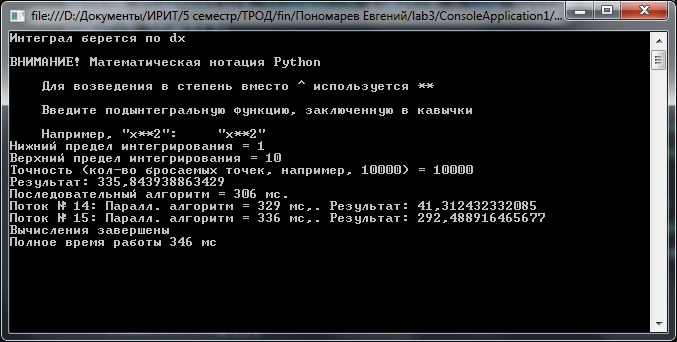
\includegraphics[scale = .8]{1_2}}
       		\caption{}
       		\label{ris:1_2}
       	\end{figure}  
       	
       	
       	     	

    \newpage    	   	
	\section{Вывод}
	В результате выполнения лабораторной работы я получил представление о возможностях библиотеки Concurrent and Coordination Runtime для организации параллельных вычислений.
	Анализируя результаты работы программы, можно выделить положительные и отрицательные стороны.
	К положительным сторонам можно отнести предоставление пользователю возможности самостоятельно задавать подынтегральную функцию любой сложности. Отрицательной особенностью выполненной реализации является скорость её работы: она примерно одинакова для каждого исполняемого вычислительного потока и практически не зависит от сложности вычислений, осуществляемых в потоке. Такое поведение обусловлено тем, что все расчеты осуществляются вызовом функции из модуля Python, что приводит к необходимости каждый раз обращаться к сеансу интерпретатора, работающего в реальном времени, то есть имеющего динамическую структуру исполнения.
	Предположительно, эти недостатки возникли из-за рассогласования используемых средств: по заданию к лабораторной работе, обязательным было условие использования библиотеки CCR для распараллеливания алгоритма. Однако, в Python так же имеются средства для реализации параллельных вычислений, и использование одного из этих подходов целостно, а не слияние двух подходов, возможно, могло бы дать выйгрыш в производительности.
		
\end{document}